\PassOptionsToPackage{table}{xcolor}
%\documentclass{beamer}
\documentclass[compress]{beamer}
%\usetheme{Epam}
\usetheme{Copenhagen}
\usepackage{xcolor}
\usepackage{listings}
\usepackage{graphicx}
\usepackage[utf8]{inputenc}
\usepackage{datetime}
\usepackage{beamerthemesplit}
%\beamertemplatenavigationsymbolsempty
\usepackage{listingsutf8}
\usepackage{ragged2e}
\usepackage{hyperref}
\lstset{ %
  language=C,                      % the language of the code
%  basicstyle=\ttfamily,           % the size of the fonts that are used for the code
%  basicstyle=\ttfamily\tiny,      % the size of the fonts that are used for the code
  basicstyle=\ttfamily\scriptsize, % the size of the fonts that are used for the code
  numbers=left,                    % where to put the line-numbers
  numberstyle=\tiny\color{gray},   % the style that is used for the line-numbers
  stepnumber=1,                    % the step between two line-numbers. If it's 1, each line 
                                   % will be numbered
  numbersep=5pt,                   % how far the line-numbers are from the code
  %backgroundcolor=\color{gray},   % choose the background color. You must add \usepackage{color}
  showspaces=false,               % show spaces adding particular underscores
  showstringspaces=false,         % underline spaces within strings
  showtabs=false,                 % show tabs within strings adding particular underscores
%  frame=shadowbox,                   % adds a frame around the code
  rulecolor=\color{black},        % if not set, the frame-color may be changed on line-breaks within not-black text (e.g. commens (green here))
  tabsize=4,                      % sets default tabsize to 4 spaces
  captionpos=,                   % sets the caption-position to bottom
  breaklines=false,                % sets automatic line breaking
  breakatwhitespace=false,        % sets if automatic breaks should only happen at whitespace
  title=\lstname,                 % show the filename of files included with \lstinputlisting;
                                  % also try caption instead of title
  keywordstyle=\color{blue},      % keyword style
  commentstyle=\color{mygreen},   % comment style
  stringstyle=\color{magenta},    % string literal style
%  escapeinside={\%*}{*)},        % if you want to add a comment within your code
  inputencoding=utf8,
  extendedchars=\true,
  morekeywords={*,..., restrict, alignof, alignas, bool, true, false, size_t, ssize_t, inline, \_Noreturn, noreturn},
  breakautoindent=false,
  breakindent=1pt,
}

%\setbeameroption{show only notes}
%\usepackage{pgfpages}
%\setbeameroption{show notes}
%\setbeameroption{show notes on second screen=right}

\setbeamertemplate{navigation symbols}{}

\definecolor{oddrow}{RGB}{100,149,237}
\definecolor{evenrow}{RGB}{135,206,250}
\def\mybs{\textbackslash}
\newcommand{\qq}{\symbol{34}} % the decimal ascii code for "
\newcommand{\sq}{\symbol{39}} % the decimal ascii code for '

\makeatletter
\newcommand{\rmnum}[1]{\romannumeral #1}
\newcommand{\Rmnum}[1]{\expandafter\@slowromancap\romannumeral #1@}
\newcommand{\inc}{\symbol{45}\symbol{45}}
\newcommand{\dec}{\symbol{43}\symbol{43}}
\newcommand{\lsh}{\symbol{60}\symbol{60}}
\newcommand{\rsh}{\symbol{62}\symbol{62}}
\makeatother

\newcommand{\specialcell}[2][c]{%
  \begin{tabular}[#1]{@{}c@{}}#2\end{tabular}}
\newcommand{\specialcellhl}[2][l]{%
  \begin{tabular}[#1]{@{}l@{}}#2\end{tabular}}
\newcommand{\specialcellhc}[2][c]{%
  \begin{tabular}[#1]{@{}c@{}}#2\end{tabular}}

\definecolor{mygreen}{rgb}{0,0.6,0}
\definecolor{olive}{rgb}{0.3, 0.4, .1}
\definecolor{fore}{RGB}{249,242,215}
\definecolor{back}{RGB}{51,51,51}
\definecolor{title}{RGB}{255,0,90}
\definecolor{dgreen}{rgb}{0.,0.6,0.}
\definecolor{gold}{rgb}{1.,0.84,0.}
\definecolor{JungleGreen}{cmyk}{0.99,0,0.52,0}
\definecolor{BlueGreen}{cmyk}{0.85,0,0.33,0}
\definecolor{RawSienna}{cmyk}{0,0.72,1,0.45}
\definecolor{Magenta}{cmyk}{0,1,0,0}

\newcommand{\kwblue}[1]{\texttt{\textcolor{blue}{#1}}}
\newcommand{\kwblack}[1]{\texttt{\textcolor{black}{#1}}}
\newcommand{\kwred}[1]{\texttt{\textcolor{red}{#1}}}
\newcommand{\kwmagenta}[1]{\texttt{\textcolor{Magenta}{#1}}}

%\newcommand{\hdr}[1]{\textless{#1}\textgreater{}}
\newcommand{\hdr}[1]{\textless{\kwmagenta{#1}}\textgreater{}}

\author[\href{mailto:vasili_slapik@epam.com}{Vasili Slapik}]{\texorpdfstring{Vasili Slapik\newline\href{mailto:vasili_slapik@epam.com}{vasili\_slapik@epam.com}}{Vasili Slapik}}


\title{Evolution of C language}
\subtitle{Overview of standards and extensions}

%TODO: _Generic with two params like generic pow(x,y)
% http://www.robertgamble.net/2012/01/c11-generic-selections.html
%
%TODO: typeof extension, very useful
%TODO: gcc ({}) block returning value, useful for macros
%TODO: pre-c11 alternative to _Static_assert

\begin{document}
%%%%%%%%%%%%%%%%%%%%%%%%%%%%%%%%%%%%%%%%%%%%%%%%%%%%%%%%%%%%%%%%%%%%%%%%%%%%%%%%%
%\setbeamertemplate{headline}{}
%\insertsectionnavigationhorizontal{.5\textwidth}{\hskip0pt plus1filll}{}
\frame{\titlepage}
%\frame{\frametitle{Table of Contents}\tableofcontents}
%\tableofcontents[
%    hideothersubsections,
%    sectionstyle=hide,
%    subsectionstyle=show,
%]
%%%%%%%%%%%%%%%%%%%%%%%%%%%%%%%%%%%%%%%%%%%%%%%%%%%%%%%%%%%%%%%%%%%%%%%%%%%%%%%%%
\begin{frame}{C main steps}
    \begin{itemize}
        \note{Miltics 1964; MIT, GE, Bell Labs; concept of file, virtual memory, dynamic linking; PL/1}
        \note{Unix end of 196x; Bell Labs; concept of file, virtual memory, dynamic linking; PL/1}
        \item 1969 - 1973: developed by Dennis Ritchie at AT\&T Bell Labs.
        \pause\item 1978: Brian Kernighan and Dennis Ritchie published the first edition of The C Programming Language. (K\&R)
        \pause\item 1989: the C standard ratified as ANSI X3.159-1989 "Programming Language C". (ANSI C or C89)
        \pause\item 1990: approved by the ISO as an international standard (C90)
        \pause\item 1999: revised standard by ISO (C99)
        \pause\item 2011: the current version approved by ISO (C11)
    \end{itemize}
\end{frame}
%%%%%%%%%%%%%%%%%%%%%%%%%%%%%%%%%%%%%%%%%%%%%%%%%%%%%%%%%%%%%%%%%%%%%%%%%%%%%%%%%
\section{C89/C90}
%%%%%%%%%%%%%%%%%%%%%%%%%%%%%%%%%%%%%%%%%%%%%%%%%%%%%%%%%%%%%%%%%%%%%%%%%%%%%%%%%
\begin{frame}{}
    \begin{block}{ \begin{Huge} \textbf{C89/C90:} \end{Huge}}
        \bigskip
        \bigskip
        \bigskip
        \begin{itemize} 
            \item GCC, Borland, Clang, Digital Mars, Watcom, MSVC, Portable C Compiler (pcc), Keil, IAR, Green Hills, IBM XL C/C++, Intel (icc) ,...
            \pause\item gcc -std=c89 -pedantic source.c
            \pause\item \_\_STDC\_\_
        \end{itemize}
        \bigskip
        \bigskip
        \bigskip
    \end{block}
\end{frame}
%%%%%%%%%%%%%%%%%%%%%%%%%%%%%%%%%%%%%%%%%%%%%%%%%%%%%%%%%%%%%%%%%%%%%%%%%%%%%%%%%
\begin{frame}{C89/C90 features}
    \begin{itemize}
        \item function prototypes (borrowed from C++)
        \pause\item keywords with corresponded semantic: \textbf{const}, \textbf{enum}, \textbf{volatile}, \textbf{void}, \textbf{signed}; \textbf{entry} keyword deleted
        \pause\item support for international character sets (wchar\_t)
        \pause\item preprocessor enhancements: \#, \#\#, \#elif, \#pragma, \#error
        \pause\item \_\_FILE\_\_, \_\_LINE\_\_, \_\_DATE\_\_, \_\_TIME\_\_
        \pause\item 8 and 9 are not octal anymore (08 and 09 are)
        \pause\item mandatory \hdr{limits.h} and \hdr{float.h}
        \pause\item formalized the C run-time library support routines
        \pause\item structures and unions can be assigned to another of the same type, passed to and returned from function
        \pause\item string literals are no longer modifiable, and so may be placed in read-only memory
        \pause\item adjacent string literals are concatenated into one string
        \pause\item hexadecimal character constants (ex.: \texttt{\mybs{x20}, \mybs{xd5}, \mybs{xff}})
    \end{itemize}
\end{frame}
%%%%%%%%%%%%%%%%%%%%%%%%%%%%%%%%%%%%%%%%%%%%%%%%%%%%%%%%%%%%%%%%%%%%%%%%%%%%%%%%%
\begin{frame}{C89/C90 features: new style of function definitions}
    K\&R function definition (the old style)
    \lstinputlisting{c89_kr_func.c}
    ANSI function definition(the new style)
    \lstinputlisting{c89_ansi_func.c}
\end{frame}
%%%%%%%%%%%%%%%%%%%%%%%%%%%%%%%%%%%%%%%%%%%%%%%%%%%%%%%%%%%%%%%%%%%%%%%%%%%%%%%%%
\begin{frame}{C89/C90 features: trigraphs}
        \begin{center}
            \only<1>{
                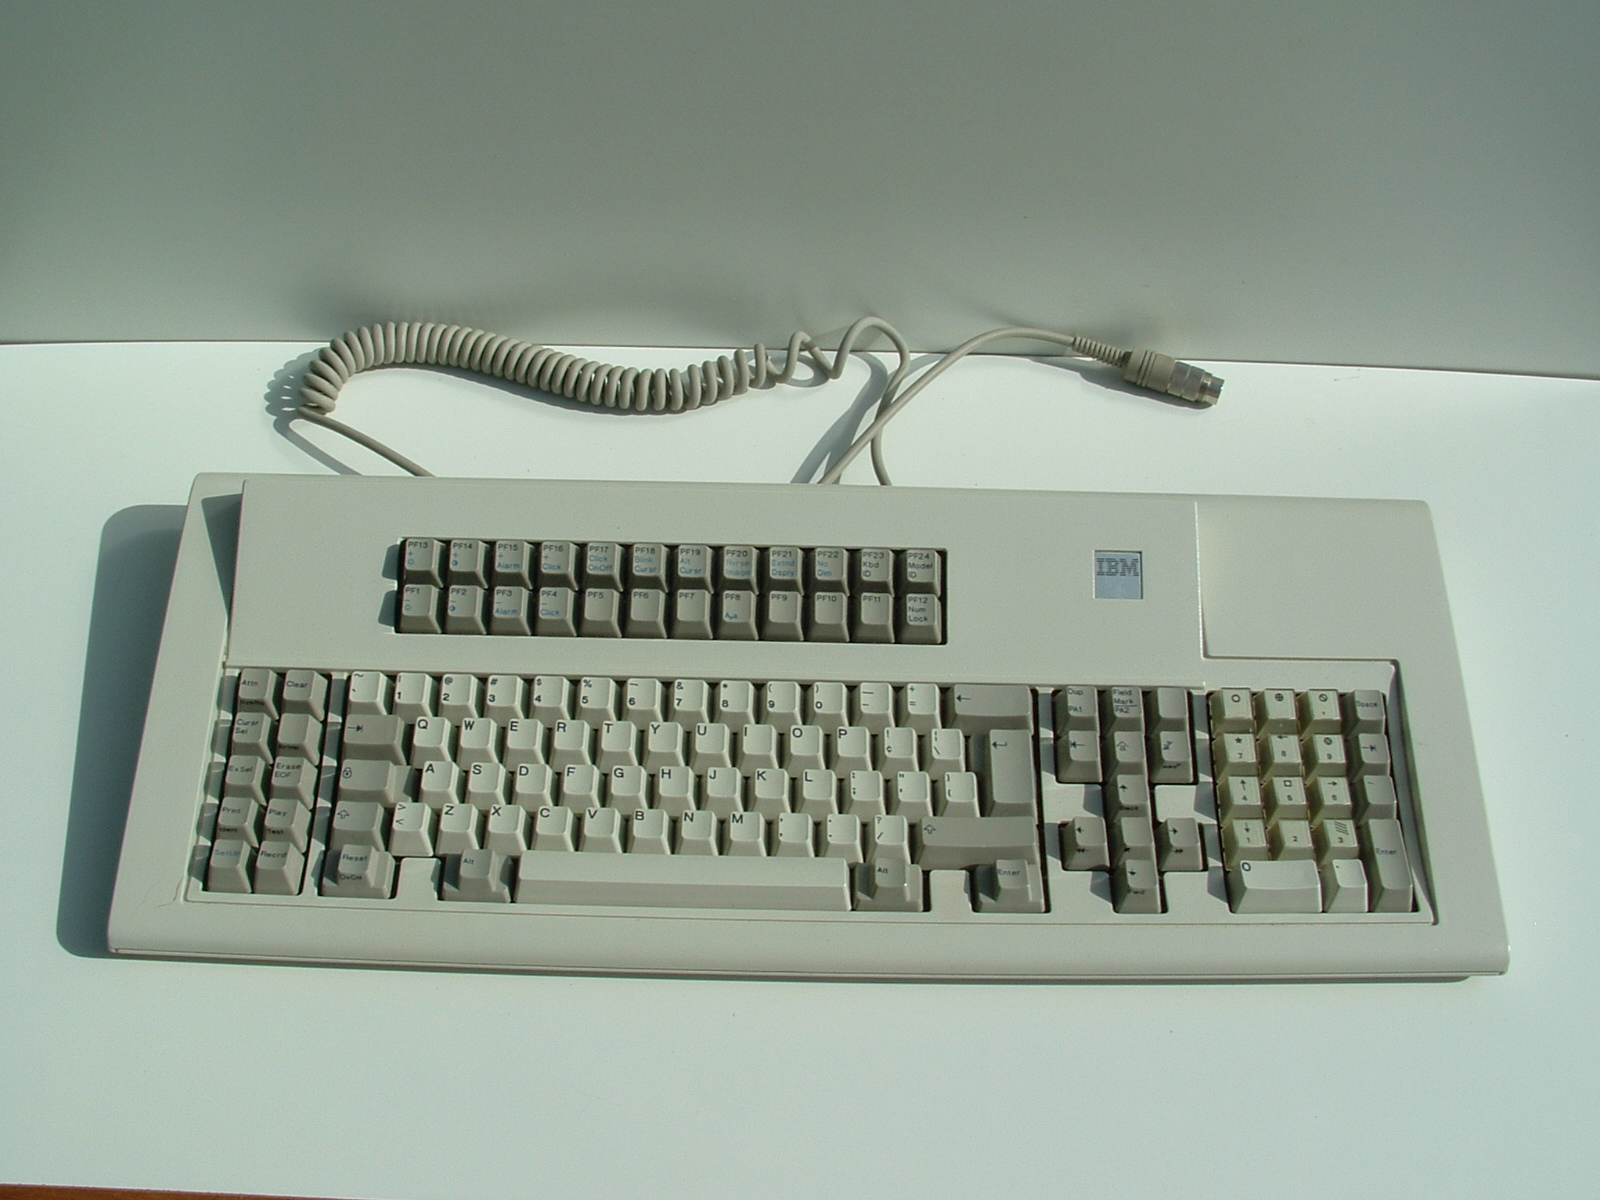
\includegraphics[height=7cm]{keybord_trigraph.jpg}
            }
            \only<2>{
                \rowcolors{1}{oddrow}{evenrow}
                \begin{tabular}{cc}
                    \textbf{trigraph}       & \textbf{replacement}      \\
                    \texttt{??=}            & \texttt{\#}               \\
                    \texttt{??(}            & \texttt{[}                \\
                    \texttt{??/}            & \texttt{\mybs}            \\
                    \texttt{??)}            & \texttt{]}                \\
                    \texttt{??'}            & \texttt{\textasciicircum} \\
                    \texttt{??\textless}    & \texttt{\textbraceleft}   \\
                    \texttt{??!}            & \texttt{\textbar}         \\
                    \texttt{??\textgreater} & \texttt{\textbraceright}  \\
                    \texttt{??-}            & \texttt{\textasciitilde}  \\
                \end{tabular}
            }
            \only<3>{
                \lstinputlisting{trigraph1.c}
            }
            \only<4>{
                \lstinputlisting{trigraph2.c}
            }
        \end{center}
\end{frame}
%%%%%%%%%%%%%%%%%%%%%%%%%%%%%%%%%%%%%%%%%%%%%%%%%%%%%%%%%%%%%%%%%%%%%%%%%%%%%%%%%
\begin{frame}{C89/C90 features: iso646.h}
    \begin{itemize}
        \item iso646.h (added in the 1995 amendment to the C89 standard)
        \begin{center}
        \rowcolors{1}{oddrow}{evenrow}
        \begin{tabular}{cc}
            \textbf{macro}          & \textbf{defined\_as}          \\
            \texttt{and}            & \texttt{\&\&}                 \\
            \texttt{and\_eq}        & \texttt{\&=}                  \\
            \texttt{bitand}         & \texttt{\&}                   \\
            \texttt{bitor}          & \texttt{\textbar}             \\
            \texttt{compl}          & \texttt{\textasciitilde}      \\
            \texttt{not}            & \texttt{!}                    \\
            \texttt{not\_eq}        & \texttt{!=}                   \\
            \texttt{or}             & \texttt{\textbar\textbar}     \\
            \texttt{or\_eq}         & \texttt{\textbar=}            \\
            \texttt{xor}            & \texttt{\^}                   \\
            \texttt{xor\_eq}        & \texttt{\textasciicircum{}=}  \\
        \end{tabular}
        \end{center}
    \end{itemize}
\end{frame}

%%%%%%%%%%%%%%%%%%%%%%%%%%%%%%%%%%%%%%%%%%%%%%%%%%%%%%%%%%%%%%%%%%%%%%%%%%%%%%%%%
\section{C99}
%%%%%%%%%%%%%%%%%%%%%%%%%%%%%%%%%%%%%%%%%%%%%%%%%%%%%%%%%%%%%%%%%%%%%%%%%%%%%%%%%
\begin{frame}{}
    \begin{block}{ \begin{Huge} \textbf{C99:} \end{Huge}}
        \bigskip
        \bigskip
        \bigskip
        \begin{itemize}
            \item GCC (mostly), Clang(mostly), IBM XL C/C++ for AIX, Pelles C, Oracle Solaris Studio
            \pause\item gcc -std=c99 -pedantic source.c
            \pause\item \_\_STDC\_VERSION\_\_ is defined with value 199901L
        \end{itemize}
        \bigskip
        \bigskip
        \bigskip
    \end{block}
\end{frame}
%%%%%%%%%%%%%%%%%%%%%%%%%%%%%%%%%%%%%%%%%%%%%%%%%%%%%%%%%%%%%%%%%%%%%%%%%%%%%%%%%
\begin{frame}{C99 features: environment}
    \begin{itemize}
        \item Increased minimum translation limits: \\
        \begin{itemize}
            \item 63 significant initial characters in an internal identifier or macro name (31 in C89)
            \item 31 significant initial characters in an external identifier (6 in C89)
            \item 4095 characters in a logical source line (509 in C89)
            \item all identifiers are case sensitive now, even external ones. (In C89, an implementation was allowed to ignore case for external identifiers.)
            \item \ldots any many other \ldots
        \end{itemize}
    \end{itemize}
\end{frame}
%%%%%%%%%%%%%%%%%%%%%%%%%%%%%%%%%%%%%%%%%%%%%%%%%%%%%%%%%%%%%%%%%%%%%%%%%%%%%%%%%
\begin{frame}{C99 features: mixed declarations and code}
    \lstinputlisting{c99_mixed_declarations_and_statements.c}
\end{frame}
%%%%%%%%%%%%%%%%%%%%%%%%%%%%%%%%%%%%%%%%%%%%%%%%%%%%%%%%%%%%%%%%%%%%%%%%%%%%%%%%%
\begin{frame}{C99 features: new block scopes for selection and iteration statements}
    \lstinputlisting{c99_for_i.c}
\end{frame}
%%%%%%%%%%%%%%%%%%%%%%%%%%%%%%%%%%%%%%%%%%%%%%%%%%%%%%%%%%%%%%%%%%%%%%%%%%%%%%%%%
\begin{frame}{C99 features: restricted pointers}
    \begin{itemize}
        \item A new keyword \textbf{restrict} was added.
        \lstinputlisting{c99_restricted_pointers.c}
    \end{itemize}
\end{frame}
%%%%%%%%%%%%%%%%%%%%%%%%%%%%%%%%%%%%%%%%%%%%%%%%%%%%%%%%%%%%%%%%%%%%%%%%%%%%%%%%%
\begin{frame}{C99 features: variable length arrays}
    \note{runtime sizeof, alloca}
    \only<1>{
        Before VLA support:
        \lstinputlisting{c99_vla1.c}
    }
    \only<2>{
        With VLA support added:
        \lstinputlisting{c99_vla2.c}
    }
    \only<3>{
        Before VLA support:
        \lstinputlisting{c99_vla3.c}
    }
    \only<4>{
        With VLA support:
        \lstinputlisting{c99_vla4.c}
    }
    \only<5>{
        \kwblue{sizeof} for VLA is \textcolor{red}{run-time} operator
    }
    \only<6>{
        \textbf{alloca} example:
        \lstinputlisting{c99_alloca.c}
    }
\end{frame}
%%%%%%%%%%%%%%%%%%%%%%%%%%%%%%%%%%%%%%%%%%%%%%%%%%%%%%%%%%%%%%%%%%%%%%%%%%%%%%%%%
\begin{frame}{C99 features:  C++ style comments}
    \lstinputlisting{c99_cpp_comments.c}
\end{frame}
%%%%%%%%%%%%%%%%%%%%%%%%%%%%%%%%%%%%%%%%%%%%%%%%%%%%%%%%%%%%%%%%%%%%%%%%%%%%%%%%%
\begin{frame}{C99 features: flexible array members}
    \note{
        About previous implementation with [0] or [1]: It's not clear if it's legal or portable,
     but it is rather popular. Official interpretation has deemed that it is not strictly conforming
     with the C Standard, although it does seem to work under all known implementations.
     (Compilers which check array bounds carefully might issue warnings.)
     }
     \note{
         As a special case, the last element of a structure with more than one named member may have
     an incomplete array type; this is called a flexible array member. In most situations, the 
     flexible array member is ignored. In particular, the size of the structure is as if the 
       flexible array member were omitted except that it may have more trailing padding than the omission would imply.
     }
    \only<1>{
        \lstinputlisting{c99_flexible_array_members.c}
    }
    \only<2>{
        \begin{itemize}
            \item Flexible array members have incomplete type, and so the \kwblue{sizeof} operator may not be applied.
            \item Flexible array members may only appear as the last member of a struct that is otherwise non-empty.
            \item A structure containing a flexible array member, or a union containing such a structure (possibly recursively), may not be a member of a structure or an element of an array.
            \item The size of the structure is as if the flexible array member was omitted
        \end{itemize}
    }
\end{frame}
%%%%%%%%%%%%%%%%%%%%%%%%%%%%%%%%%%%%%%%%%%%%%%%%%%%%%%%%%%%%%%%%%%%%%%%%%%%%%%%%%
\begin{frame}{C99 features: complex numbers}
    \only<1>{
        \begin{itemize}
            \item New keywords \kwblue{\_Complex} and \kwblue{\_Imaginary} were added, the header \hdr{complex.h} defines correspondingly \kwblue{complex} and \kwblue{imaginary} definition.
            \item There are three complex types, corresponding to the three real types: \kwblue{float complex}, \kwblue{double complex}, and \kwblue{long double complex}
            \item To construct complex numbers \hdr{complex.h} defines two macros that can be used to create complex numbers:  \textbf{\_Complex\_I} and \textbf{I}.
            \item Additional functions were added: \textbf{cimag, creal, carg, conj, cproj, cabs, cexp, clog, cpow, csqrt, cacos, casin, catan, ccos, csin, ctan, cacosh, casinh, catanh, ccosh, csinh, ctanh}
        \end{itemize}
    }
    \only<2>{
        \lstinputlisting{c99_complex.c}
    }
\end{frame}
%%%%%%%%%%%%%%%%%%%%%%%%%%%%%%%%%%%%%%%%%%%%%%%%%%%%%%%%%%%%%%%%%%%%%%%%%%%%%%%%%
\begin{frame}{C99 features: \_\_func\_\_ predefined identifier}
    \lstinputlisting{c99__func__macro.c}
\end{frame}
%%%%%%%%%%%%%%%%%%%%%%%%%%%%%%%%%%%%%%%%%%%%%%%%%%%%%%%%%%%%%%%%%%%%%%%%%%%%%%%%%
\begin{frame}{C99 features: digraphs (1993 AM1)}
    \begin{center}
        \rowcolors{1}{oddrow}{evenrow}
        \begin{tabular}{cc}
            \textbf{digraph}        & \textbf{replacement}      \\
            \texttt{\textless:}     & \texttt{[}                \\
            \texttt{:\textgreater}  & \texttt{]}                \\
            \texttt{\textless\%}    & \texttt{\textbraceleft}   \\
            \texttt{\%\textgreater} & \texttt{\textbraceright}  \\
            \texttt{\%:}            & \texttt{\#}               \\
        \end{tabular}
    \end{center}
\end{frame}
%%%%%%%%%%%%%%%%%%%%%%%%%%%%%%%%%%%%%%%%%%%%%%%%%%%%%%%%%%%%%%%%%%%%%%%%%%%%%%%%%
\begin{frame}{C99 features: relaxed constraints on aggregate and union initialization}
    \only<1>{
        \begin{block}{\textbf{C89}}
        All the expressions in an initializer for an object that has static
        storage duration \colorbox{yellow}{or in an initializer list for an object that has
        aggregate or union} type shall be constant expressions
        \end{block}
        \begin{block}{\textbf{C99}}
        All the expressions in an initializer for an object that has static
        storage duration shall be constant expressions or string literals
        \end{block}
    }
    \only<2>{
        \lstinputlisting{c99_relaxed_constr.c}
    }
\end{frame}
%%%%%%%%%%%%%%%%%%%%%%%%%%%%%%%%%%%%%%%%%%%%%%%%%%%%%%%%%%%%%%%%%%%%%%%%%%%%%%%%%
\begin{frame}{C99 features: designated initializers}
    \lstinputlisting{c99_designated_initializers.c}
\end{frame}
%%%%%%%%%%%%%%%%%%%%%%%%%%%%%%%%%%%%%%%%%%%%%%%%%%%%%%%%%%%%%%%%%%%%%%%%%%%%%%%%%
\begin{frame}{C99 features: compound literals}
    \lstinputlisting{c99_compound_literals.c}
\end{frame}
%%%%%%%%%%%%%%%%%%%%%%%%%%%%%%%%%%%%%%%%%%%%%%%%%%%%%%%%%%%%%%%%%%%%%%%%%%%%%%%%%
\begin{frame}{C99 features: type generic math tgmath.h}
    \only<1>{
        \begin{itemize}
            \item The \hdr{tgmath.h} header includes the headers \hdr{math.h} and \hdr{complex.h}
             and defines several type-generic macros.  These macros determines the actual
             function to call depending on the types of the parameters.
        \end{itemize}
    }
    \only<2>{
        \begin{center}
            \rowcolors{1}{oddrow}{evenrow}
            \scalebox{0.63}{
                \begin{tabular}{ccccccc}
                    \textbf{macro} & \textbf{float} & \textbf{double} & \textbf{long double} & \textbf{float} &  \textbf{double} & \textbf{long double} \\
                    asin & asinf & asin & \text{asinl} & casinf & casin & casinl \\
                    acos & acosf & acos & acosl & cacosf & cacos & cacosl \\
                    atan & atanf & atan & atanl & catanf & catan & catanl \\
                    asinh & asinhf & asinh & asinhl & casinhf & casinh & casinhl \\
                    acosh & acoshf & acosh & acoshl & cacoshf & cacosh & cacoshl \\
                    atanh & atanhf & atanh & atanhl & catanhf & catanh & catanhl \\
                    sin & sinf & sin & sinl & csinf & csin & csinl \\
                    cos & cosf & cos & cosl & ccosf & ccos & ccosl \\
                    tan & tanf & tan & tanl & ctanf & ctan & ctanl \\
                    sinh & sinhf & sinh & sinhl & csinhf & csinh & csinhl \\
                    cosh & coshf & cosh & coshl & ccoshf & ccosh & ccoshl \\
                    tanh & tanhf & tanh & tanhl & ctanhf & ctanh & ctanhl \\
                    exp & expf & exp & expl & cexpf & cexp & cexpl \\
                    log & logf & log & logl & clogf & clog & clogl \\
                    pow & powf & pow & powl & cpowf & cpow & cpowl \\
                    sqrt & sqrtf & sqrt & sqrtl & csqrtf & csqrt & csqrtl \\
                    abs & fabsf & fabs & fabsl & cabsf & cabs & cabsl \\
                    exp & expf & exp & expl & cexpf & cexp & cexpl \\
                \end{tabular}
            }
        \end{center}
    }
    \only<3>{
        \begin{center}
            \rowcolors{1}{oddrow}{evenrow}
            \scalebox{0.63}{
                \begin{tabular}{cccccccc}
                    \textbf{macro} & \textbf{float} & \textbf{double} & \textbf{long double} & \textbf{macro} & \textbf{float} &  \textbf{double} & \textbf{long double} \\
                    atan2 & atan2f & atan2 & atan2l & llrint & llrintf & llrint & llrintl \\
                    cbrt & cbrtf & cbrt & cbrtl & llround & llroundf & llround & llroundl \\
                    ceil & ceilf & ceil & ceill & log10 & log10f & log10 & log10l \\
                    copysign & copysignf & copysign & copysignl & log1p & log1pf & log1p & log1pl \\
                    erf & erff & erf & erfl & log2 & log2f & log2 & log2l \\
                    erfc & erfcf & erfc & erfcl & logb & logbf & logb & logbl \\
                    exp2 & exp2f & exp2 & exp2l & lrint & lrintf & lrint & lrintl \\
                    expm1 & expm1f & expm1 & expm1l & lround & lroundf & lround & lroundl \\
                    fdim & fdimf & fdim & fdiml & nearbyint & nearbyintf & nearbyint & nearbyintl \\
                    floor & floorf & floor & floorl & nextafter & nextafterf & nextafter & nextafterl \\
                    fma & fmaf & fma & fmal & nexttoward & nexttowardf & nexttoward & nexttowardl \\
                    fmax & fmaxf & fmax & fmaxl & remainder & remainderf & remainder & remainderl \\
                    fmin & fminf & fmin & fminl & remquo & remquof & remquo & remquol \\
                    fmod & fmodf & fmod & fmodl & rint & rintf & rint & rintl \\
                    frexp & frexpf & frexp & frexpl & round & roundf & round & roundl \\
                    hypot & hypotf & hypot & hypotl & scalbln & scalblnf & scalbln & scalblnl \\
                    ilogb & ilogbf & ilogb & ilogbl & scalbn & scalbnf & scalbn & scalbnl \\
                    ldexp & ldexpf & ldexp & ldexpl & tgamma & tgammaf & tgamma & tgammal \\
                    lgamma & lgammaf & lgamma & lgammal & trunc & truncf & trunc & truncl \\
                \end{tabular}
            }
        \end{center}
    }
    \only<4>{
        \scalebox{0.8}{
            \lstinputlisting{c99_tgmath.c}
        }
    }
    \only<5>{
        \scalebox{0.9}{
            \lstinputlisting[basicstyle=\ttfamily\tiny]{c99_tgmath2.c}
        }
    }
\end{frame}
%%%%%%%%%%%%%%%%%%%%%%%%%%%%%%%%%%%%%%%%%%%%%%%%%%%%%%%%%%%%%%%%%%%%%%%%%%%%%%%%%
\begin{frame}{C99 features: remove implicit int}
    \only<1>{
        \note{Broke backward compatibility}
        \lstinputlisting{c99_implicit_int.c}
    }
    \only<2>{
        \note{Valid even in C++}
        \lstinputlisting{c99_implicit_int2.c}
    }
    \only<3>{
        \note{Because the compiler assumes that foo() returns a value of type int for this noncompliant code example, UINT_MAX is incorrectly converted to −1.}
        \lstinputlisting{c99_implicit_int3.c}
    }
\end{frame}
%%%%%%%%%%%%%%%%%%%%%%%%%%%%%%%%%%%%%%%%%%%%%%%%%%%%%%%%%%%%%%%%%%%%%%%%%%%%%%%%%
\begin{frame}{C99 features: remove implicit function declaration}
    \only<1>{
        \begin{block}{\textbf{C89}}
        If the expression that precedes the parenthesized argument list in a function 
        call consists solely of an identifier, and if no declaration is visible for this identifier, 
        the identifier is implicitly declared exactly as if, in the innermost block containing the 
        function call, the declaration \textbf{extern int identifier();} appeared.
        \end{block}
    }
    \only<2>{
        \lstinputlisting[firstline=2]{c99_remove_implicit_function_declaration.c}
    }
\end{frame}
%%%%%%%%%%%%%%%%%%%%%%%%%%%%%%%%%%%%%%%%%%%%%%%%%%%%%%%%%%%%%%%%%%%%%%%%%%%%%%%%%
\begin{frame}{C99 features: allows trailing comma in enum declaration}
    \scalebox{0.8}{
        \lstinputlisting{c99_comma.c}
    }
\end{frame}
%%%%%%%%%%%%%%%%%%%%%%%%%%%%%%%%%%%%%%%%%%%%%%%%%%%%%%%%%%%%%%%%%%%%%%%%%%%%%%%%%
\begin{frame}{C99 features: boolean type}
    \only<1>{
        \begin{itemize}
            \item A new keyword \kwblue{\_Bool}
            \item A new header file \hdr{stdbool.h}
        \end{itemize}
    }
    \only<2>{
        \begin{block}{ \textbf{C99}}
            When any scalar value is converted to \kwblue{\_Bool}, the result is 0 if the value compares equal to 0; otherwise, the result is 1
        \end{block}
        \bigskip
        \bigskip
            \lstinputlisting{c99_bool3.c}
    }
%    \only<3>{
%        \scalebox{0.8}{
%            \lstinputlisting{c99_bool2.c}
%        }
%    }
\end{frame}
%%%%%%%%%%%%%%%%%%%%%%%%%%%%%%%%%%%%%%%%%%%%%%%%%%%%%%%%%%%%%%%%%%%%%%%%%%%%%%%%%
\begin{frame}{C99 features: \_Pragma preprocessing operator}
    \lstinputlisting{c99_pragma.c}
\end{frame}
%%%%%%%%%%%%%%%%%%%%%%%%%%%%%%%%%%%%%%%%%%%%%%%%%%%%%%%%%%%%%%%%%%%%%%%%%%%%%%%%%
\begin{frame}{C99 features: hexadecimal floating-point constants and printf/scanf specifiers}
    \lstinputlisting{c99_hex_fp_constants.c}
\end{frame}
%%%%%%%%%%%%%%%%%%%%%%%%%%%%%%%%%%%%%%%%%%%%%%%%%%%%%%%%%%%%%%%%%%%%%%%%%%%%%%%%%
\begin{frame}{C99 features: miscelanious features}
    \begin{itemize}
        \item inline functions
        \pause\item \kwblue{long long int} and library functions
    \end{itemize}
\end{frame}
%%%%%%%%%%%%%%%%%%%%%%%%%%%%%%%%%%%%%%%%%%%%%%%%%%%%%%%%%%%%%%%%%%%%%%%%%%%%%%%%%
\section{C11}
%%%%%%%%%%%%%%%%%%%%%%%%%%%%%%%%%%%%%%%%%%%%%%%%%%%%%%%%%%%%%%%%%%%%%%%%%%%%%%%%%
\begin{frame}{}
    \begin{block}{ \begin{Huge} \textbf{C11:} \end{Huge}}
        \bigskip
        \bigskip
        \bigskip
        \begin{itemize}
            \item GCC (partly), Clang(mostly), Peles C
            \pause\item gcc -std=c11 -pedantic source.c
            \pause\item \_\_STDC\_VERSION\_\_ definded as 201112L
        \end{itemize}
        \bigskip
        \bigskip
        \bigskip
    \end{block}
\end{frame}
%%%%%%%%%%%%%%%%%%%%%%%%%%%%%%%%%%%%%%%%%%%%%%%%%%%%%%%%%%%%%%%%%%%%%%%%%%%%%%%%%
%\begin{frame}{C11 features: quick\_exit and at\_quick\_exit functions}
%    \lstinputlisting{c11_quick_exit.c}
%\end{frame}
%%%%%%%%%%%%%%%%%%%%%%%%%%%%%%%%%%%%%%%%%%%%%%%%%%%%%%%%%%%%%%%%%%%%%%%%%%%%%%%%%
\begin{frame}{C11 features: \_Noreturn keyword}
    \only<1>{
        \lstinputlisting{c11_noreturn.c}
    }
    \only<2>{
        \begin{itemize}
            \item longjmp()
            \item abort()
            \item exit()
            \item \_Exit()
            \item quick\_exit()
        \end{itemize}
    }
    \only<3>{
        \begin{itemize}
            \item \hdr{stdnoreturn.h}: \\
                \texttt{\#define noreturn \_Noreturn}
        \end{itemize}
    }
    \only<4>{
        \begin{itemize}
            \item gcc equivalent
            \lstinputlisting{c11_noreturn_gcc.c}
        \end{itemize}
    }
\end{frame}
%%%%%%%%%%%%%%%%%%%%%%%%%%%%%%%%%%%%%%%%%%%%%%%%%%%%%%%%%%%%%%%%%%%%%%%%%%%%%%%%%
\begin{frame}{C11 features: alignment specification}
    \only<1>{
        \begin{itemize}
            \item \hdr{stdalign.h} header
                \lstinputlisting{c11_stdalign.c}
        \end{itemize}
    }
    \only<2>{
        \begin{itemize}
            \item \textbf{alignof} operator
                \lstinputlisting{c11_alignof.c}
        \end{itemize}
    }
    \only<3>{
        \begin{itemize}
            \item \textbf{alignas} operator
                \lstinputlisting{c11_alignas.c}
        \end{itemize}
    }
    \only<4>{
        \begin{itemize}
            \item\textbf{alignas}
                \begin{itemize}
                    \item the \textbf{alignas} specifier cannot reduce alignment
                    \item requested alignment should be a power of 2
                    \item an alignment specification of zero has no effect
                    \item when multiple alignments are specified, the strictest takes effect
                \end{itemize}
         \end{itemize}
    }
    \only<5>{
        \begin{itemize}
           \item\textbf{max\_align\_t} is usually synonymous with the largest scalar type, which is \textbf{long double} on most platforms
            \lstinputlisting[firstline=2]{c11_max_align_t.c}
        \end{itemize}
    }
    \only<6>{
        \begin{itemize}
            \item \textbf{aligned\_alloc} function in \hdr{stdlib.h}
                \lstinputlisting{c11_aligned_alloc.c}
        \end{itemize}
    }
\end{frame}
%%%%%%%%%%%%%%%%%%%%%%%%%%%%%%%%%%%%%%%%%%%%%%%%%%%%%%%%%%%%%%%%%%%%%%%%%%%%%%%%%
\begin{frame}{C11 features: type-generic expressions using the \_Generic keyword}
    \lstinputlisting{c11_generic.c}
\end{frame}
%%%%%%%%%%%%%%%%%%%%%%%%%%%%%%%%%%%%%%%%%%%%%%%%%%%%%%%%%%%%%%%%%%%%%%%%%%%%%%%%%
\begin{frame}{C11 features: anonymous structures and unions}
    \lstinputlisting{c11_anon.c}
\end{frame}
%%%%%%%%%%%%%%%%%%%%%%%%%%%%%%%%%%%%%%%%%%%%%%%%%%%%%%%%%%%%%%%%%%%%%%%%%%%%%%%%%
\begin{frame}{C11 features: static assertion}
    \lstinputlisting{c11_static_assertion.c}
\end{frame}
%%%%%%%%%%%%%%%%%%%%%%%%%%%%%%%%%%%%%%%%%%%%%%%%%%%%%%%%%%%%%%%%%%%%%%%%%%%%%%%%%
\begin{frame}{C11 features: an exclusive create-and-open mode ("...x") for fopen}
    POSIX version: O\_CREAT|O\_EXCL
    \lstinputlisting{c11_fopenx.c}
\end{frame}
%%%%%%%%%%%%%%%%%%%%%%%%%%%%%%%%%%%%%%%%%%%%%%%%%%%%%%%%%%%%%%%%%%%%%%%%%%%%%%%%%
\begin{frame}{C11 features: bound-checking interfaces (Annex K) }
    \only<1>{
        \_\_STDC\_LIB\_EXT1\_\_
    }
    \only<2>{
        \begin{itemize}
            \item\textbf{gets\_s, getenv\_s, wctomb\_s, mbstowcs\_s, wcstombs\_s, memcpy\_s, memmove\_s, strcpy\_s, strncpy\_s, strcat\_s, strncat\_s, strerror\_s, strnlen\_s, wcscpy\_s, wcsncpy\_s, wmemcpy\_s, wmemmove\_s, wcscat\_s, wcsncat\_s, wcsnlen\_s, wcrtomb\_s, mbsrtowcs\_s, wcsrtombs\_s}
        \lstinputlisting{c11_bound_checking.c}
        \end{itemize}
    }
    \only<3>{
        \begin{itemize}
            \item \textbf{memset\_s}: the standard guarantees that \textbf{memset\_s} will overwrite the argument array
        \end{itemize}
    }
    \only<4>{
        \begin{itemize}
            \item new \textbf{printf}
                \lstinputlisting{c11_printf_s.c}
            \begin{itemize}
                \item \textbf{format} shall not be a null pointer
                \item \textbf{\%n} shall not appear in the string pointed to by \textbf{format}
                \item if there is a runtime-constraint violation, the \textbf{printf\_s} function does not attempt to
                produce further output
            \end{itemize}
        \end{itemize}
    }
    \only<5>{
        \begin{itemize}
            \item extra argument \textbf{context} for \textbf{bsearch\_s, qsort\_s}
                \scalebox{0.9}{
                    \lstinputlisting{c11_bound_checking_context.c}
                 }
        \end{itemize}
    }
\end{frame}
%%%%%%%%%%%%%%%%%%%%%%%%%%%%%%%%%%%%%%%%%%%%%%%%%%%%%%%%%%%%%%%%%%%%%%%%%%%%%%%%%
\begin{frame}{C11 features: concurrency}
    \begin{itemize}

        \only<1>{
            \item macros:
                \begin{itemize}
                    \item thread\_local
                    \item ONCE\_FLAG
                    \item TSS\_DTOR\_ITERATIONS
                    \item cnd\_t
                    \item thrd\_t
                    \item tss\_t
                    \item mtx\_t
                    \item tss\_dtor\_t
                    \item thrd\_start\_t
                    \item once\_flag
                \end{itemize}

            \item enumeration constants to pass to mtx\_init:
                \begin{itemize}
                     \item mtx\_plain
                     \item mtx\_recursive
                     \item mtx\_timed
                \end{itemize}
        }

        \only<2>{
            \item enumeration constants for threads
                \begin{itemize}
                    \item thrd\_timedout
                    \item thrd\_success
                    \item thrd\_busy
                    \item thrd\_error
                    \item thrd\_nomem
                \end{itemize}

            \item functions for condition variables:
                \begin{itemize}
                    \item call\_once(once\_flag *flag, void (*func)(void));
                    \item cnd\_broadcast(cnd\_t *cond);
                    \item cnd\_destroy(cnd\_t *cond);
                    \item cnd\_init(cnd\_t *cond);
                    \item cnd\_signal(cnd\_t *cond);
                    \item cnd\_timedwait(cnd\_t *restrict cond, mtx\_t *restrict mtx, const struct timespec *restrict ts);
                    \item cnd\_wait(cnd\_t *cond, mtx\_t *mtx);
                \end{itemize}
        }

        \only<3>{
            \item the mutex functions:
                \begin{itemize}
                    \item void mtx\_destroy(mtx\_t *mtx);
                    \item int mtx\_init(mtx\_t *mtx, int type);
                    \item int mtx\_lock(mtx\_t *mtx);
                    \item int mtx\_timedlock(mtx\_t *restrict mtx, const struct timespec *restrict ts);
                    \item int mtx\_trylock(mtx\_t *mtx);
                    \item int mtx\_unlock(mtx\_t *mtx);
                \end{itemize}

            \item thread functions:
                \begin{itemize}
                    \item int thrd\_create(thrd\_t *thr, thrd\_start\_t func, void *arg);
                    \item thrd\_t thrd\_current(void);
                    \item int thrd\_detach(thrd\_t thr);
                    \item int thrd\_equal(thrd\_t thr0, thrd\_t thr1);
                    \item noreturn void thrd\_exit(int res);
                    \item int thrd\_join(thrd\_t thr, int *res);
                    \item int thrd\_sleep(const struct timespec *duration, struct timespec *remaining);
                    \item void thrd\_yield(void);
                \end{itemize}
        }

        \only<4>{
            \item thread-specific storage functions:
                \begin{itemize}
                    \item int tss\_create(tss\_t *key, tss\_dtor\_t dtor);
                    \item void tss\_delete(tss\_t key);
                    \item void *tss\_get(tss\_t key);
                    \item int tss\_set(tss\_t key, void *val);
                \end{itemize}
        }

        \only<5>{
            \item TinyCThread, Pelles C
            \item \_\_STDC\_NO\_THREADS\_\_
        }

    \end{itemize}
\end{frame}
%%%%%%%%%%%%%%%%%%%%%%%%%%%%%%%%%%%%%%%%%%%%%%%%%%%%%%%%%%%%%%%%%%%%%%%%%%%%%%%%%
\begin{frame}{C11 features: miscelanious features}
    \begin{itemize}
        \item \textbf{gets} removed
        \pause\item improved Unicode support based on the C Unicode Technical Report ISO/IEC TR 19769:2004:
            \begin{itemize}
                \item \textbf{char16\_t} and \textbf{char32\_t} types for storing UTF-16/UTF-32 encoded data including conversion functions in <uchar.h>
                \item the corresponding u and U string literal prefixes, as well as the u8 prefix for UTF-8 encoded literals
            \end{itemize}
        \pause\item macros for the construction of complex values
            \lstinputlisting{c11_cmplx.c}
    \end{itemize}
\end{frame}

%%%%%%%%%%%%%%%%%%%%%%%%%%%%%%%%%%%%%%%%%%%%%%%%%%%%%%%%%%%%%%%%%%%%%%%%%%%%%%%%%
%\begin{frame}{C11 features: UTF-8 string literals}
%    \lstinputlisting{c11_utf8.c}
%\end{frame}
%%%%%%%%%%%%%%%%%%%%%%%%%%%%%%%%%%%%%%%%%%%%%%%%%%%%%%%%%%%%%%%%%%%%%%%%%%%%%%%%%
\begin{frame}{C11 features, GCC support status}
    \begin{center}
        \rowcolors{1}{oddrow}{evenrow}
        \begin{tabular}{lc}
            -std=c1x & GCC 4.6 \\
            -std=c11 & GCC 4.7 \\
            \_\_STDC\_VERSION\_\_ == 201112L & GCC 4.7 \\
            \_Alignas, \_Alignof, max\_align\_t, stdalign.h & GCC 4.7 \\
            \_Atomic, stdatomic.h & GCC 4.9 \\
            \_Generic & GCC 4.9 \\
            \_Noreturn, stdnoreturn.h & GCC 4.7 \\
            \_Static\_assert & GCC 4.6 \\
            \_Thread\_local & GCC 4.9 \\
            Anonymous struct and union & GCC 4.6 \\
%            Typedef redefinition & GCC 4.6 \\
%            New macros in float.h & GCC 4.6 \\
            Unicode strings & GCC 4.7 \\
        \end{tabular}
    \end{center}
\end{frame}
%%%%%%%%%%%%%%%%%%%%%%%%%%%%%%%%%%%%%%%%%%%%%%%%%%%%%%%%%%%%%%%%%%%%%%%%%%%%%%%%%
\section{GCC extentions}
%%%%%%%%%%%%%%%%%%%%%%%%%%%%%%%%%%%%%%%%%%%%%%%%%%%%%%%%%%%%%%%%%%%%%%%%%%%%%%%%%
\begin{frame}{gcc extentions: labels as values}
    \lstinputlisting{gcc_labels_as_values.c}
\end{frame}
%%%%%%%%%%%%%%%%%%%%%%%%%%%%%%%%%%%%%%%%%%%%%%%%%%%%%%%%%%%%%%%%%%%%%%%%%%%%%%%%%
\begin{frame}{gcc extentions: nested functions}
    \lstinputlisting{gcc_nested_functions.c}
\end{frame}
%%%%%%%%%%%%%%%%%%%%%%%%%%%%%%%%%%%%%%%%%%%%%%%%%%%%%%%%%%%%%%%%%%%%%%%%%%%%%%%%%
\begin{frame}{gcc extentions: case ranges}
    \lstinputlisting{gcc_case_ranges.c}
\end{frame}
%%%%%%%%%%%%%%%%%%%%%%%%%%%%%%%%%%%%%%%%%%%%%%%%%%%%%%%%%%%%%%%%%%%%%%%%%%%%%%%%%
\begin{frame}{gcc extentions: binary constants}
    \lstinputlisting{gcc_binary_constants.c}
\end{frame}
%%%%%%%%%%%%%%%%%%%%%%%%%%%%%%%%%%%%%%%%%%%%%%%%%%%%%%%%%%%%%%%%%%%%%%%%%%%%%%%%%
\end{document}
